Ein wichtiger Bestandteil jeder Software ist das Logging von unterschiedlichen Ereignissen.
Das Ziel vom Logging ist später von den Softwareentwicklern verschiedene Fehler in der Software so schnell wie möglich zu finden und
zu beseitigen.

Dafür muss es möglich sein mit den Logs die Fehler so genau wie möglich in der Software zu lokalisieren 
(welche Komponente oder welche Methode den Fehler hervorgerufen hat) 
und welche Ereigniskette den jeweiligen Fehler hervorgerufen hat.

In dem Kapitel \ref{kap:Dataflow} sind alle möglichen Wege basierend auf der beschriebenen Struktur 
im Kapitel \ref{kap:Structur} für die ankommenden Ereignissen in der Software beschrieben.

Die nachfolgende Abbildung \ref{fig:FullDataFlow} zeigt den kompletten Ablauf beim Geschehen eines Ereignisses.
Eine mögliche Systematisierung des Loggings in der Appliaction wäre: 
\begin{itemize}
    \item Aufzeichnung des Inhaltes des ankommenden Ereignisses in jeder Komponente
    \item Aufzeichnung des Inhaltes des ausgehenden Ereignisses in jeder Komponente 
    \item Aufzeichnung aller Komponenten, an die das Ereignis weitergegeben wird
\end{itemize}

Somit lassen sich die Fehler auf die Komponente genau lokalisieren, d.h. es lässt sich ein entsprechender Unittest schreiben, 
der diesen Fehler abdeckt. Auch ein Integrationtest ist möglich, da der Ablauf des Ereignisses ebenfalls bekannt ist.


\begin{figure}[H]
    \centering
    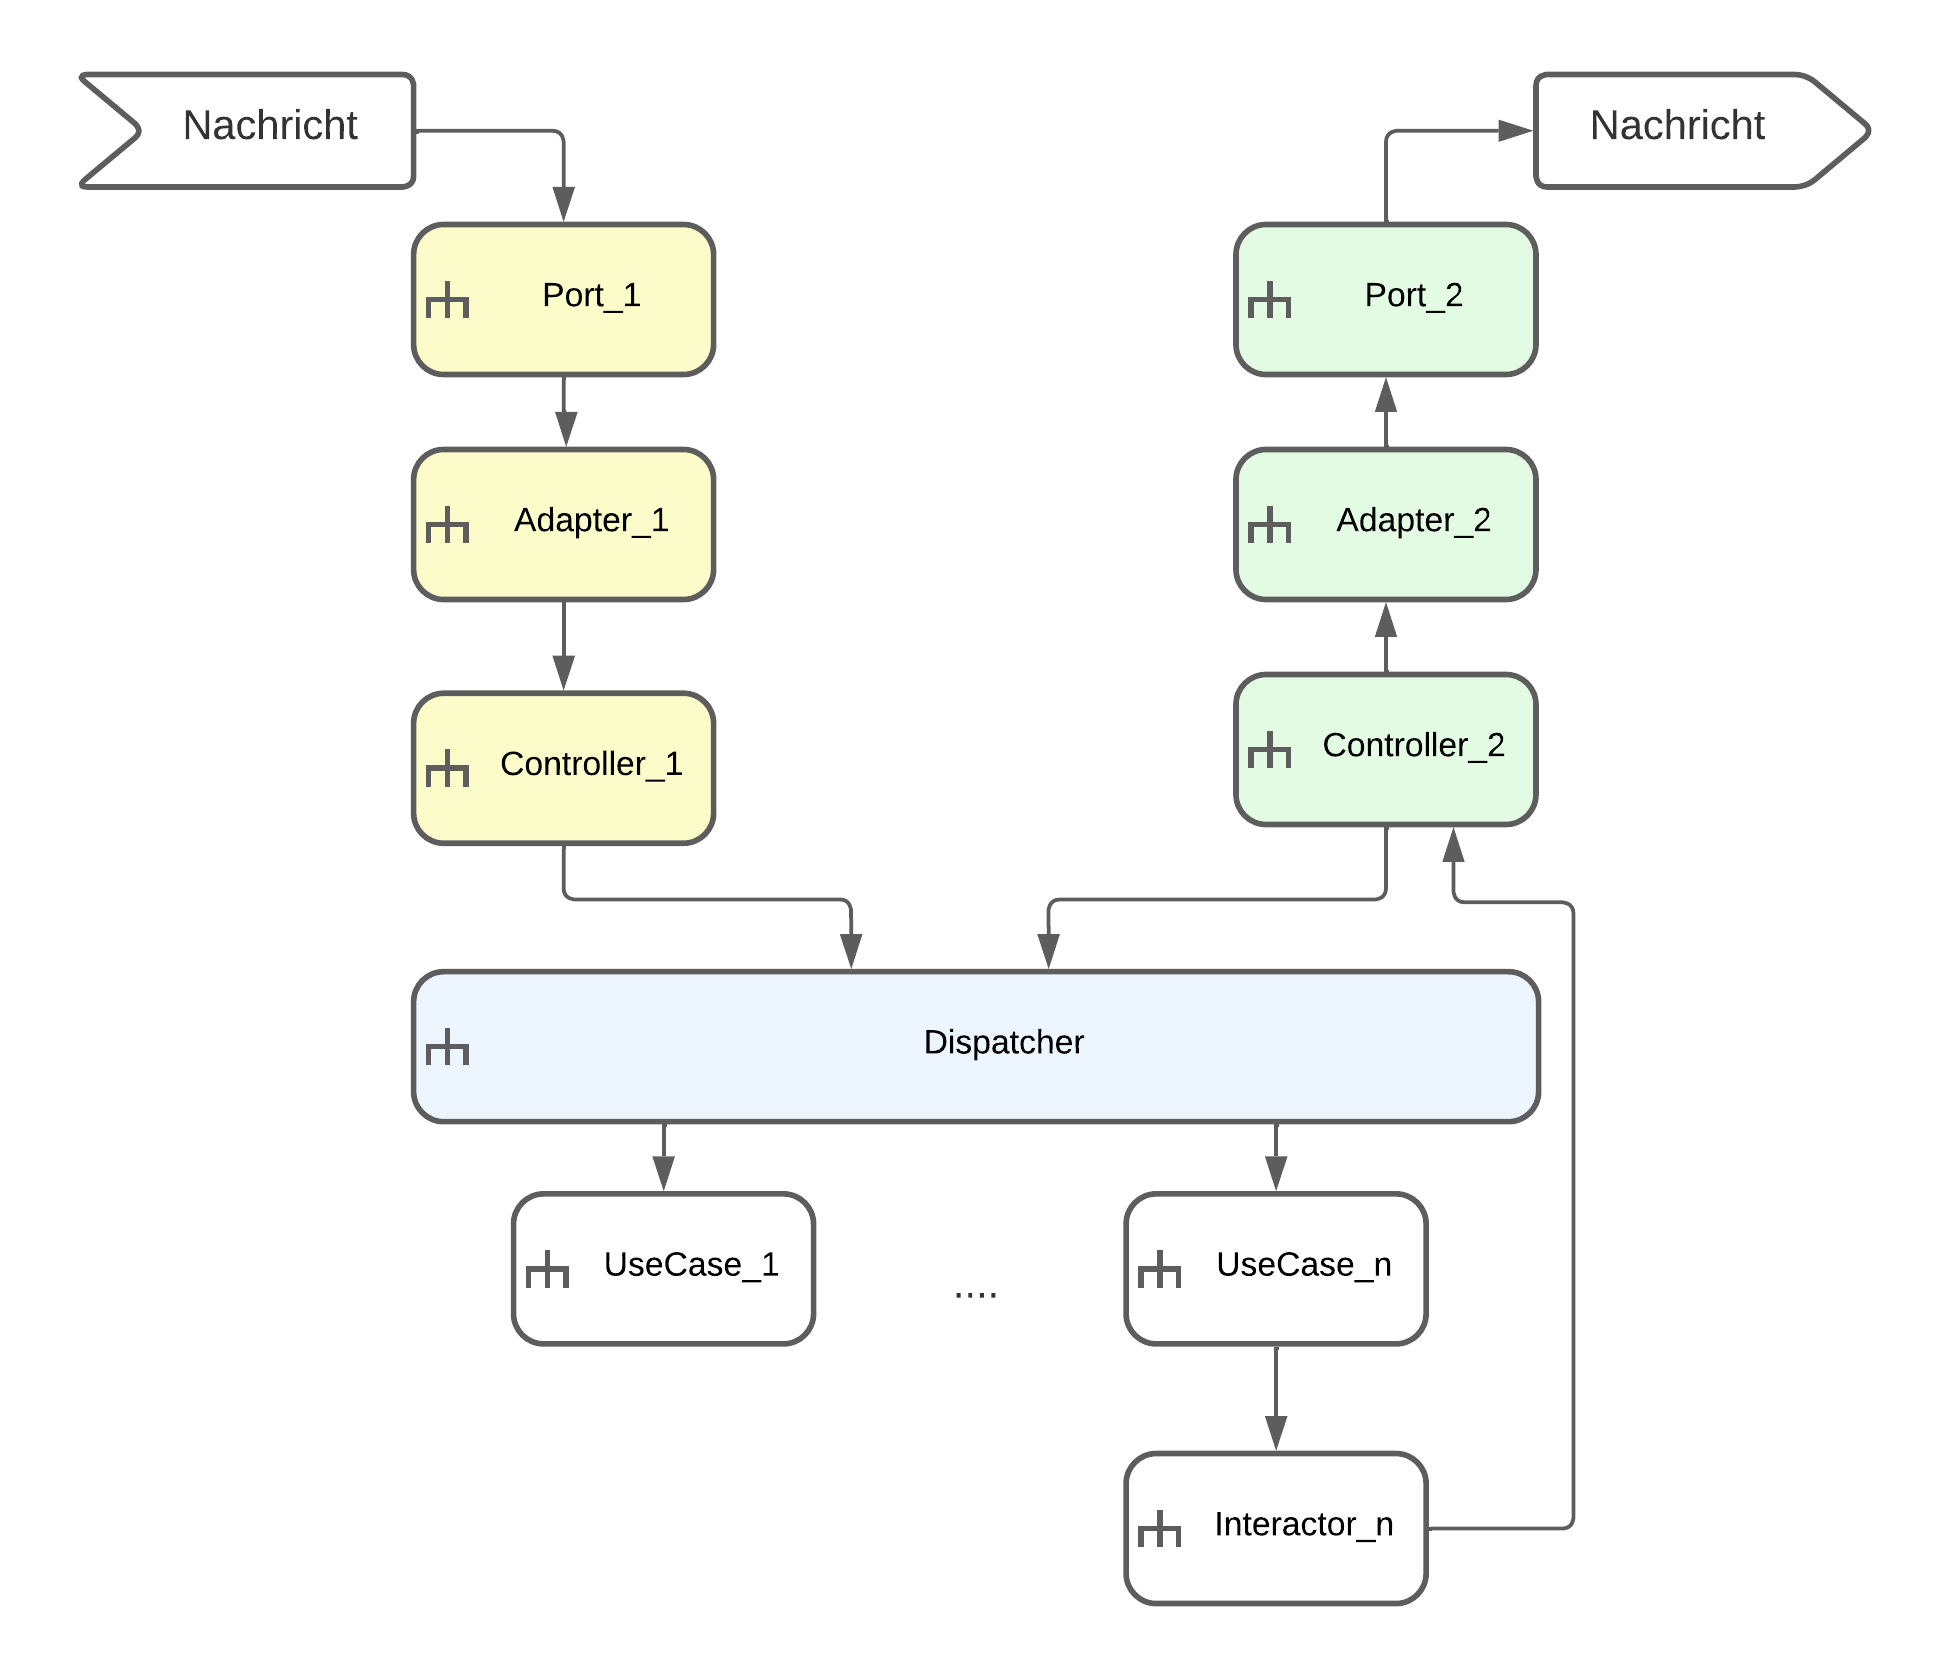
\includegraphics[width=12cm]{./images/FullDataFlow.png}
     \caption[Kompletter Datenfluss]{Kompletter Datenfluss}
     \label{fig:FullDataFlow}
\end{figure}
